\begin{figure}[!htb] 
    \centering
    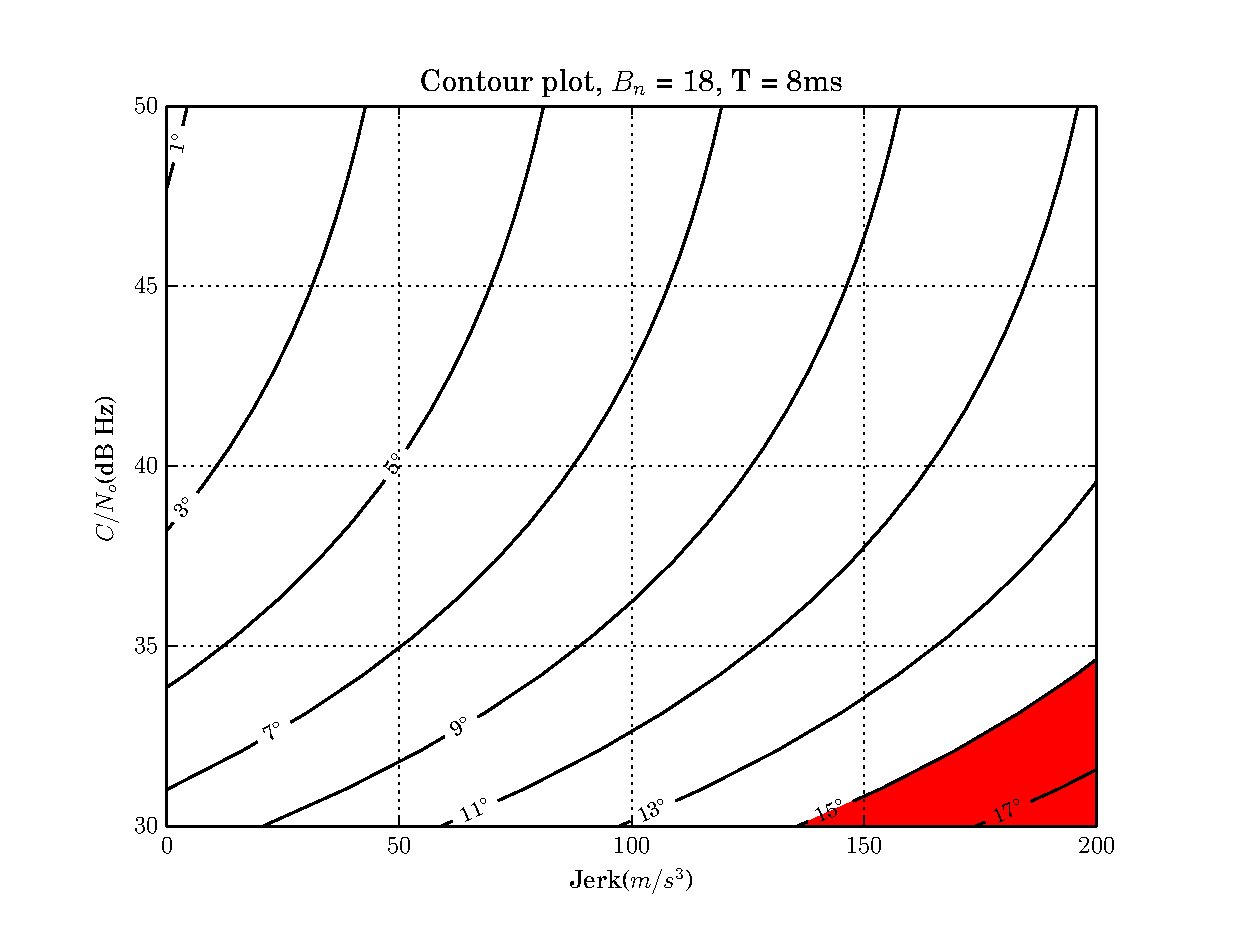
\includegraphics[width=1\textwidth]{mywork/18.eps} 
    \caption{}
\end{figure}

\begin{figure}[!htb] 
    \centering
    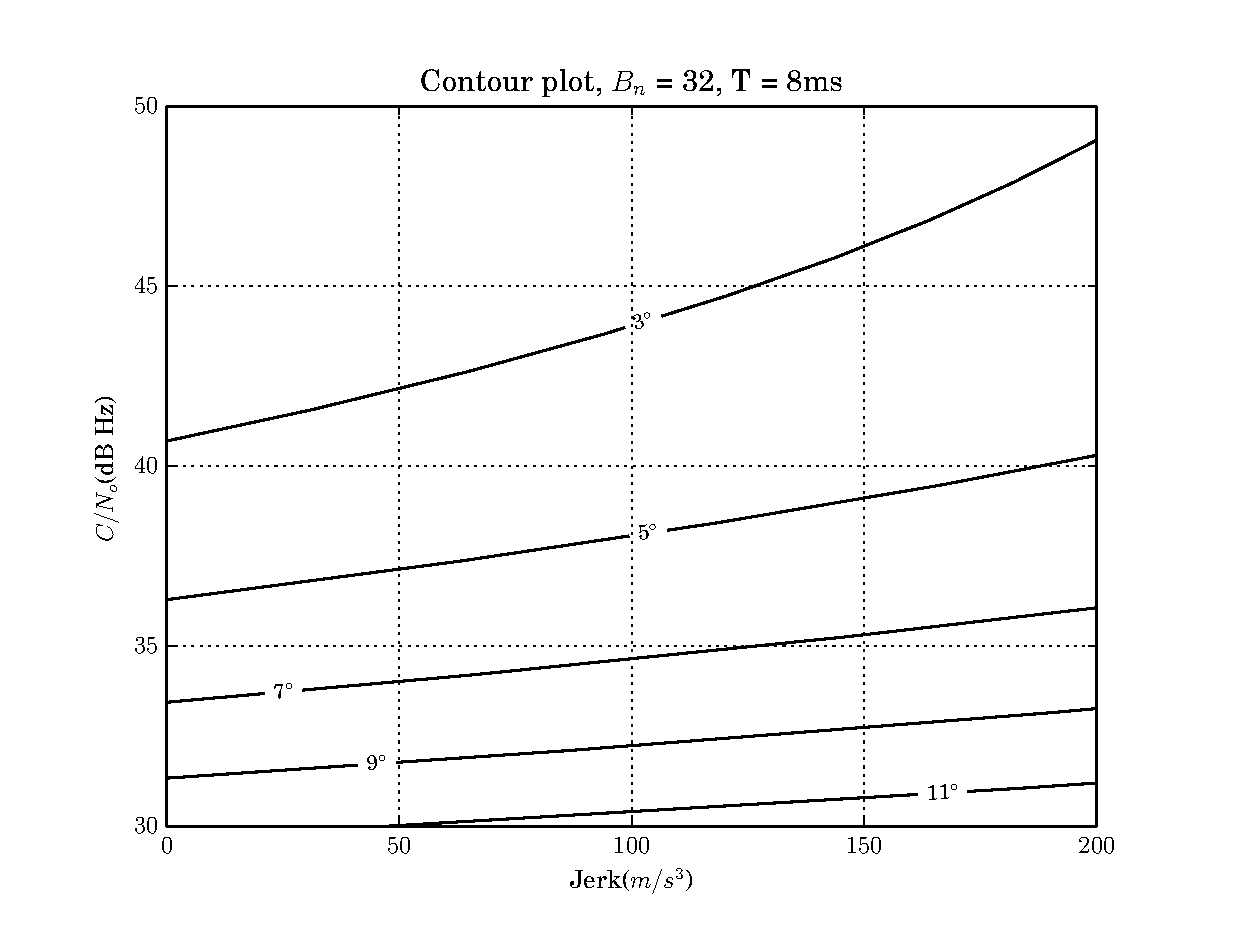
\includegraphics[width=1\textwidth]{mywork/32.eps} 
    \caption{}
\end{figure}


\begin{figure}[!htb] 
    \centering
    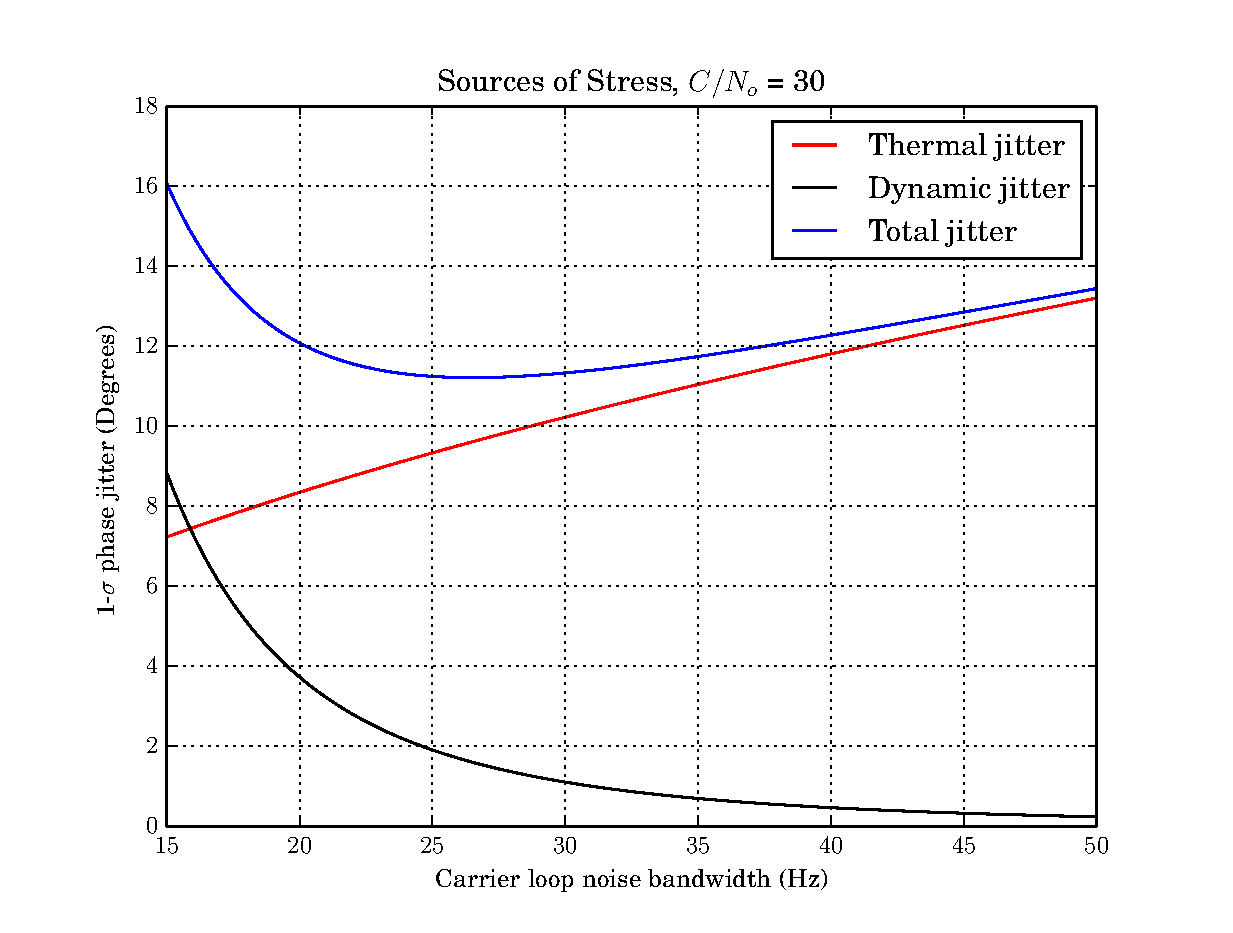
\includegraphics[width=1\textwidth]{mywork/Stresses.eps} 
    \caption{}
\end{figure}





\section{Kaplan Stuff}
Kaplan suggests that "A conservative rule of thumb for tracking threshold is that the 3-sigma jitter must not exceed one-fourth of the phase pull-in range of the PLL discriminator." %\cite{Kaplan}

\begin{equation}
3 \sigma_{PLL} = 3 \sigma_j +\theta_e \leq 45 \degree
\end{equation}

Where:
\begin{align*}
\sigma_j &= \text{1-sigma phase jitter from all sources except dynamic stress error} \\
\theta_e &= \text{dynamic stress error in the PLL tracking loop}
\end{align*}


%\cite{Kaplan}

Equation 5.5
\begin{equation}
\sigma_{PLL} = \sqrt{\sigma^2_{tPLL} + \sigma^2_v+ \theta^2_A} + \frac{\theta_e}{3} \leq 15 \degree 
\end{equation}
%\cite{Jwo}

Where:
\begin{align*}
\sigma_{tPLL} &= \text{1-sigma thermal noise in degrees}\\
\sigma_v &= \text{1-sigma vibration-induced oscillator jitter in degrees}\\
\theta_A &= \text{Allan variance induced oscillator jitter in degrees}
\end{align*}



%\cite{Kaplan}\cite{Jwo}

Equation 5.6
\begin{equation}
\sigma_{PLLt} = \frac{360}{2 \pi} \sqrt{\frac{B_n}{C/N_0}(1+\frac{1}{2TC/N_0})} (degrees)
\end{equation}
%\cite{Kaplan}





Talk about this
5.6.2 FLL Tracking Loop Measurement Errors

Generate figure 5.24
Generate figure 5.25

Also talk about section 5.6.2








\begin{comment}

\chapter{Preliminary Work}\label{ch:PreliminaryWork}
Significant preliminary work has been carried out, because of the challenging scope of thesis. 

In order to have a rigorous understanding of the dynamic performance of the Namuru receiver, we must first examine the theoretical basis for the operation of its tracking loops. 

A model of the operation of the tracking loops can be established by building upon intellectual foundations laid in continuous time control theory. While this Laplace domain model provides an idealised understanding of the \ac{PLL}, it does not take into the effects of delay and jitter in the loop. 

\ac{PLL}, \ac{FLL} and \ac{DLL} are all examples of control systems. By convention, what is referred to in the parlance of control theory as a "controller" is referred to as the "loop filter" in \ac{GNSS} related literature. One key point to keep in mind with a \ac{PLL} is that a phase input results in a frequency output. This effective integration occurs in the \ac{VCO}.

\section{Current Namuru architecture}
A significant amount of time has been spent gaining an understanding of the Namuru receiver, its architecture and the operation of it's sub-systems. The receiver is a mixed signal device, which has been the focus of a decade of research and development. 

A thorough understanding of the receiver's operation is critical, because one of the ways the receiver diverts from an idealised model is because of the jitter and delays introduced by its \ac{RTOS}. Hence, a detailed understanding of the receiver is crucial, if it is to be accurately modeled. 

The Aquarius firmware developed by Glennon \cite{Glennon11aquariusfirmware} ultimately implements the tracking loop algorithm. The implementation of purely the tracking loop is 4,100 lines of optimised C, illustrating the complexity of the implementation.

The Namuru receiver currently uses a third-order \ac{PLL} loop filter with a second-order \ac{FLL} assist. This architecture can be seen in figure \ref{fig:Architecture}.  A third order \ac{PLL} uses a second order filter, with the third integrator being the \ac{VCO}.

After conducting a literature review, the first task was to replicate the Laplace domain models of the control loops, used in the Namuru receiver, so that the receiver can be modelled in the Laplace domain. The choice of the coefficients from the tracking loop comes from a method devised by Ward \cite{Ward}. While this method is conceptually simple, requiring only a loop order and noise bandwidth as parameters, it generates robust tracking loops for most applications. 

\section{\ac{FLL} Filter}
In the Laplace domain, we can represent the second order \ac{FLL} filter as as :  $F(s) = K_1 + \frac{K_2}{s}$. The design method from Ward \cite{Ward} is used in order to determine the coefficients $K_1$ and $K_2$.  

$$B_n = 6$$
$$a_2 = \sqrt(2)$$
$$\omega_{0}=\frac{B_n}{0.53}$$

\begin{equation} \label{eq1}
\begin{split}
K_1 & = a_2 \times \omega_{0}\\
K_1 & = 16.0099648571\\
\end{split}
\end{equation}

\begin{equation} \label{eq2}
\begin{split}
K_2 & = \omega_{0}^2\\
K_2 & = 128.159487362\\
\end{split}
\end{equation}

\begin{figure}[!htb] 
    \centering
    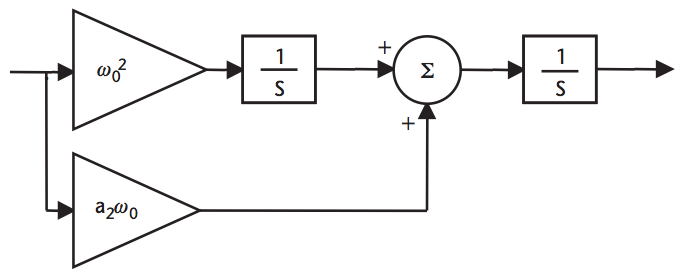
\includegraphics[width=1\textwidth]{mywork/SecondOrderLoop.png} 
    \caption{The architecture of the \ac{FLL} filter implemented in Namuru, the integrator on the right represents the \ac{VCO}. Image from \cite{Kaplan}}
    \label{fig:SecondOrderLoop}
\end{figure}


\section{\ac{PLL} Filter}
Ward's method is also used to design the co-efficients for the \ac{PLL}. In the Laplace domain, we can represent the second order filter  of the third order \ac{PLL} as : 

\begin{equation} \label{eq6}
F(s) = K_1 + \frac{K_2}{s} + \frac{K_3}{s^2}
\end{equation}

A loop bandwidth of 18 was chosen for the \ac{PLL}, as Kaplan\cite{Kaplan} demonstrated, using a Monte Carlo simulation, that higher loops bandwidths typically result in unstable behaviour. 
Using Ward's method\cite{Ward} for finding $K_1,K_2\&K_3$:

$$B_n = 18$$
$$a_3=1.1$$
$$b_3=2.4$$
$$\omega_{0}=\frac{B_n}{0.7845}$$

\begin{equation} \label{eq3}
\begin{split}
K_1 & = b_3 \times \omega_{0}\\
    & = 55.0669216061\\
\end{split}
\end{equation}

\begin{equation} \label{eq4}
\begin{split}
K_2 & = a_3 \times \omega_{0}^2\\ 
    & = 579.097645953\\
\end{split}
\end{equation}

\begin{equation} \label{eq5}
\begin{split}
K_3 & = \omega_{0}^3\\
    & = 12079.2138909\\
\end{split}
\end{equation}


The next stage of Laplace domain analysis after determining the transfer function of the filter is to determine the transfer function of the closed loop system.

Multiplying equation \ref{eq6} by $\frac{s^2}{s^2}$ we get :

\begin{equation}
F(s) = \frac{K_1s^2 + K_2^s + K_3}{s^2}
\end{equation}

The \ac{VCO} has the following transfer function : $G(s) = \frac{K_{vco}}{s}$

From Kazemi, if  $F(s)$ is the transfer function of the loop filter\cite{KazemiPHD} then the closed loop transfer function  of the system is: 

\begin{equation}
 H(s) = \frac{K_{VCO}F(s)}{s+K_{VCO}F(s)}
\end{equation}

\begin{equation}
 H(s) = \frac{K_{VCO}(K_1 + \frac{K_2}{s} + \frac{K_3}{s^2})}{s+K_{VCO}(K_1 + \frac{K_2}{s} + \frac{K_3}{s^2})}
\end{equation}

Multiplying by $\frac{s^2}{s^2}$ we get :

\begin{equation}
 H(s) = \frac{K_{VCO}(K_1s^2 + K_2s + K_3)}{s^3+K_{VCO}(K_1s^2 + K_2s + K_3)}
 \end{equation}

\begin{figure}[!htb] 
    \centering
    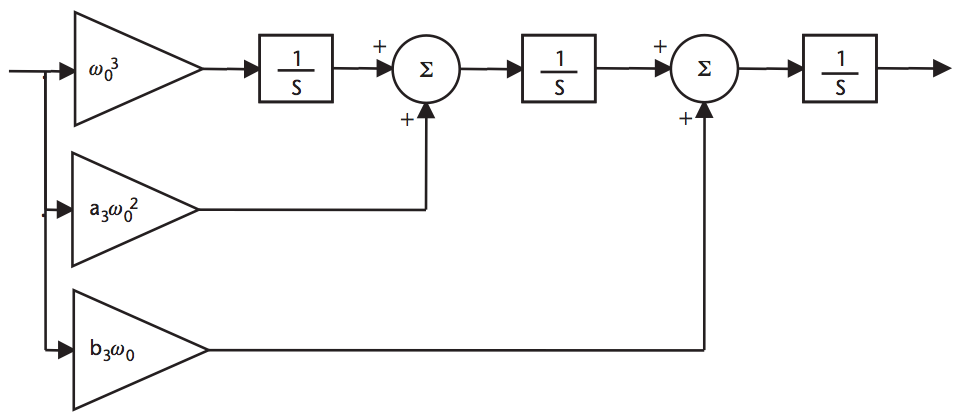
\includegraphics[width=1\textwidth]{mywork/ThirdOrderLoop.png} 
    \caption{The architecture of the PLL filter,the integrator on the right represents the VCO. Image from \cite{Kaplan}}
    \label{fig:ThirdOrderLoop}
\end{figure}

\section{Zeros and Poles}
The behaviour of a closed loop system is determined by the locations of the zeros and the poles. In particular, their location determines if the system is stable for all possible inputs. Even if the system is found not to be stable for all possible inputs, it may be stable for all \emph{reasonable} inputs. An important caveat is that the location of the zeros and poles is for an analog model of the system, the locations will be different for a digital model, with the difference in location depending on the $B_LT$ product.  Hence it is possible to design a system which is stable in the Laplace domain but unstable in the Z Domain. 

Root locus provides an efficient graphical method for analysing the stability of a system in the Laplace domain\cite{Nise}. Matlab was used to generate a Root Locus plot of the current Laplace domain model of the \ac{PLL} implementation using the following code:

\begin{lstlisting}[frame=single]
Kvco =1;
Bn = 18;
a3 = 1.1;
b3 = 2.4;
omega = Bn/0.7845;
k1 = b3*omega;
k2 = a3*(omega^2);
k3 = omega^3;
%H is the forward transfer function
H = tf([Kvco*k1 Kvco*k2 Kvco*k3],[1 0 0 0]);
rlocus(H);
\end{lstlisting}

The results of this analysis can be seen in figure \ref{fig:RootLocus}, from this analysis of the root locus, we can determine  that the system is stable, for values of the $V_CO$ gain which are larger than 0.38. This is an important result, as intuitively, increasing the gain will typically make a system unstable. However, this result demonstrates the value of Root Locus analysis for evaluating the stability of a higher order system.

\begin{figure}[!htb] 
    \centering
    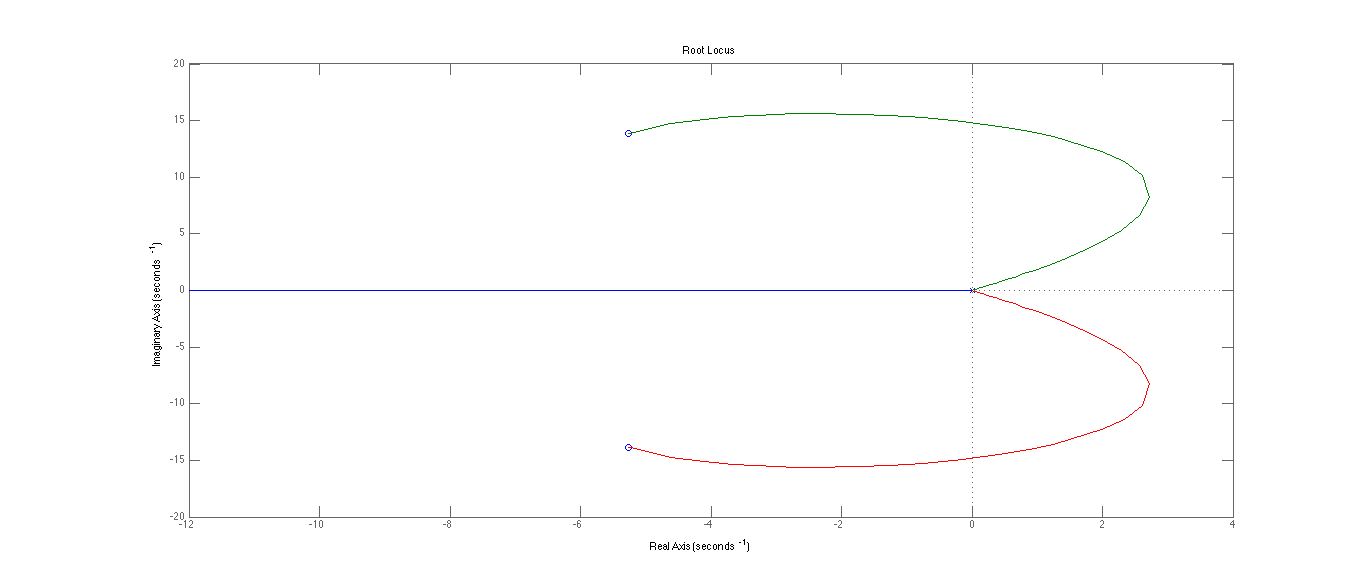
\includegraphics[width=1\textwidth]{mywork/RootLocus.png} 
    \caption{Root Locus of the Analog model of the Namuru Phase Locked Loop. The root locus intersects the imaginary axis when the gain is 0.38.}
    \label{fig:RootLocus}
\end{figure}


In order to verify the implementation of the analog model was correct, a second graphical model was constructed in CircuitLab. This model can be seen in figure \ref{fig:gpsLoopModel}. By adjusting the VCO gain, the threshold between stable and unstable behaviour for a step input was confirmed to be 0.38. The results from this experiment can be seen in figures \ref{fig:Stable} and \ref{fig:Unstable}

\begin{figure}[!htb] 
    \centering
    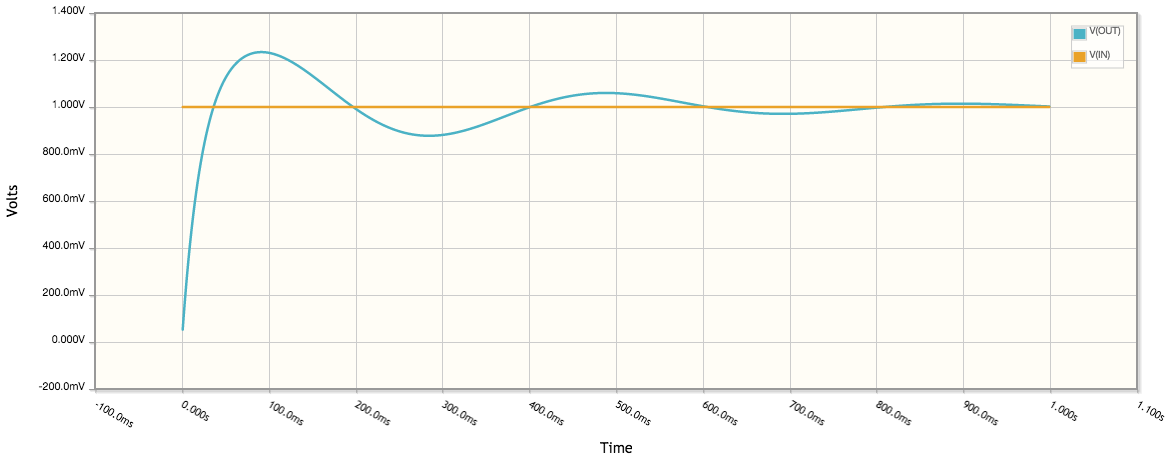
\includegraphics[width=1\textwidth]{mywork/Stable.png} 
    \caption{Step response to the \ac{PLL} model for a VCO gain of 1.}
    \label{fig:Stable}
\end{figure}

\begin{figure}[!htb] 
    \centering
    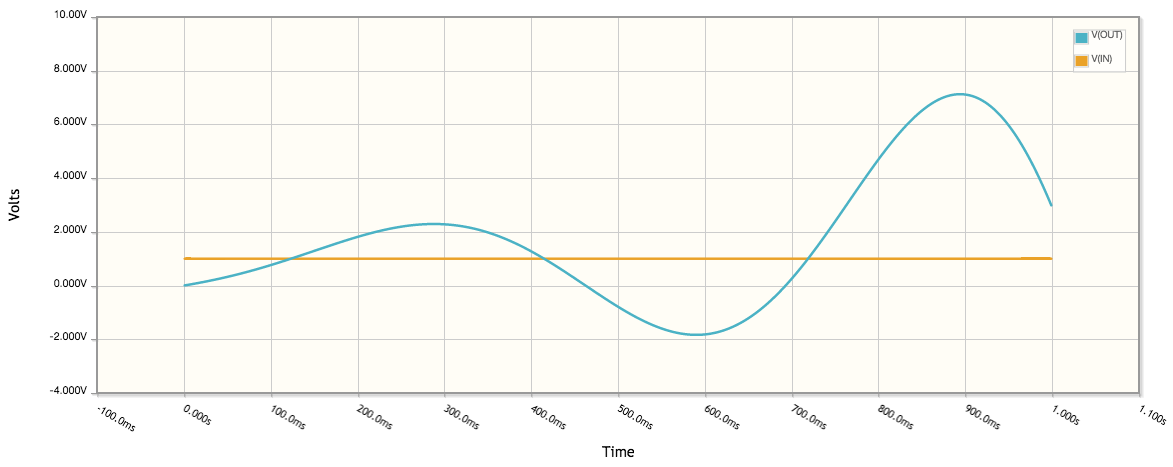
\includegraphics[width=1\textwidth]{mywork/Unstable.png} 
    \caption{Step response to the \ac{PLL} model for a VCO gain of 0.1, the system is clearly unstable.}
    \label{fig:Unstable}
\end{figure}

Additionally, this model confirmed that the currentNamuru architecture is able to integrate up velocity and acceleration however it is vulnerable to Jerk. This was assessed by applying ramp and parabolic inputs to the input, and comparing to the output.

\begin{figure}[!htb] 
    \centering
    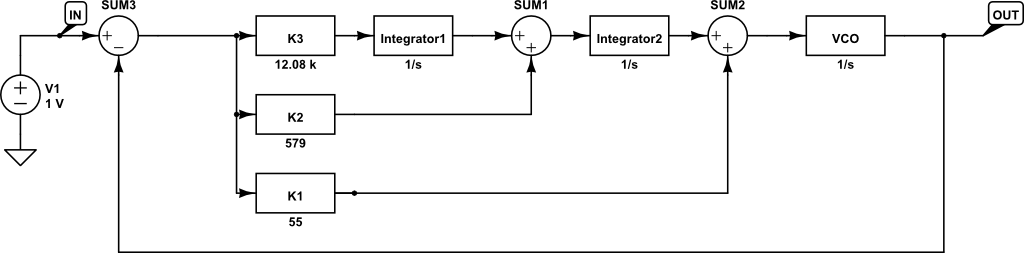
\includegraphics[width=1\textwidth]{mywork/gpsLoopModel.png} 
    \caption{A graphical Laplace domain model of the currently implemented \ac{PLL} in the Namuru receiver.}
    \label{fig:gpsLoopModel}
\end{figure}

\section{Simulation}

The sophisticated method of modelling the performance of the tracking loops is using a computer simulation. A software based receiver has been developed as part of the thesis, in order to gain a greater understanding of the performance of tracking loops on real world data. 

The software receiver was developed in python, based on the authors previous experience processing GNSS data using the language. For the receiver, the software architecture described by Kai Borre et al in \cite{KaiBorre} was used as a reference, however with significant modifications in order to improve the clarity of the operation of the tracking loop. The approach of using an \ac{GNSS}, and testing in software was effectively used by Kazemi \cite{KazemiPHD} in order to critically evaluate the performance of the new tracking loops developed as part of his PHD. The code included in Appendix 3 includes an implementation of the tracking loops as developed by Spliker \cite{Spilker}.

Synthetic data was created using software, and a signal was generated by a Spirent \ac{GPS} simulator. This signal was then digitised using a NordNav \ac{SDR}, with a sampling rate of $16.3676 \times 10^6$ samples per second. An example of a Spirent \ac{GPS} simulator can be seen in figure \ref{fig:Spirent}.

A range of simulations were created in order to better understand the performance of the software receiver. In particular, scenarios for 0g, 1g, 2g, 5g, 7.5g and 10g were created. In figure \ref{fig:Doppler}, the output from the \ac{NCO} of the software receiver can be seen. In the simulation, the receiver remains stationary until 8s, at which point it starts acceleration directly upwards at 10g, creating a ramp in the \ac{NCO} frequency. It is important to note that while the receiver is accelerating at 10g, the \ac{LOS} dynamics may only be 5g. 

\begin{figure}[!htb] 
    \centering
    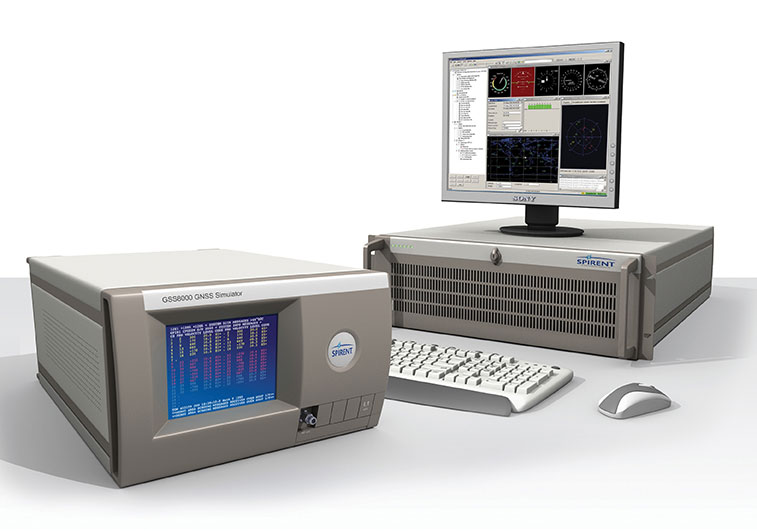
\includegraphics[width=1\textwidth]{mywork/Spirent-GSS8000.jpg} 
    \caption{An example of a Spirent \ac{GPS} simulator. The actual model used differs from the one pictured.}
    \label{fig:Spirent}
\end{figure}

\begin{figure}[!htb] 
    \centering
    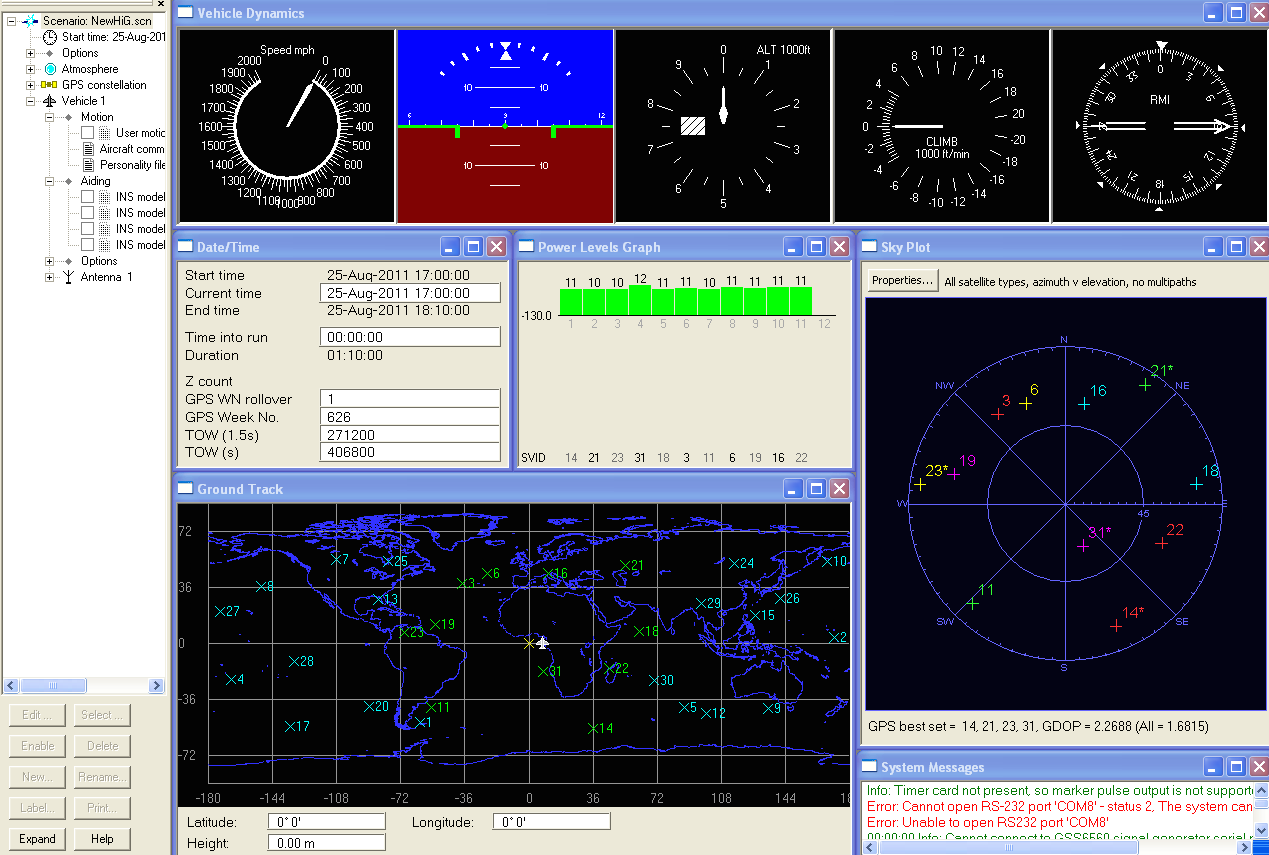
\includegraphics[width=1\textwidth]{mywork/HighGScreenshot.png} 
    \caption{The SimGen software, used to define scenarios and control the \ac{GNSS} simulator.}
    \label{fig:HighGScreenshot}
\end{figure}


The correct performance of a \ac{PLL} can be examined by attempting to decode the navigation message transmitted by the satellite. Other, more sophisticated methods for determining if the receiver is in phase lock, will be examined in Thesis B. In figures \ref{fig:RawSignal} and \ref{fig:DigitalSignal}, the decoded message can be clearly seen, indicating that the receiver is maintaining phase lock with the signal.

\begin{figure}[!htb] 
    \centering
    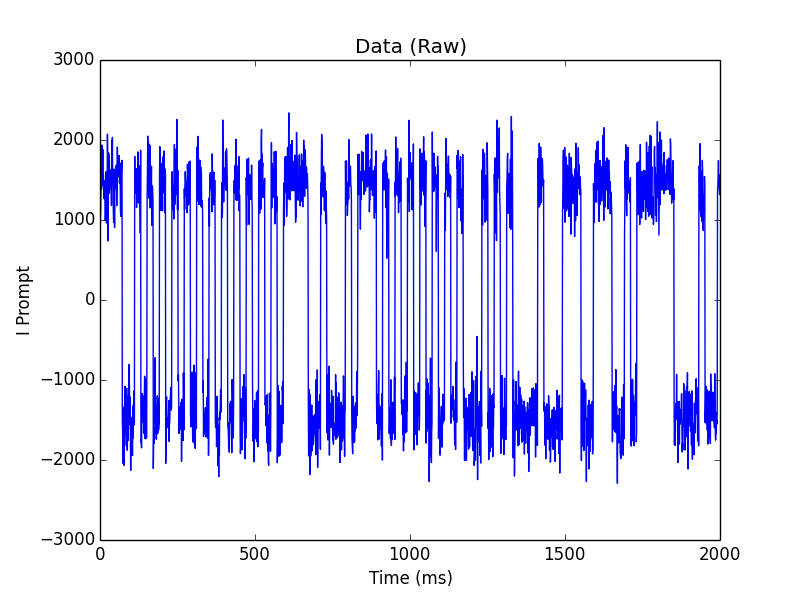
\includegraphics[width=1\textwidth]{mywork/3Raw.png} 
    \caption{The raw signal captured by the software receiver, the integration period is 1ms.}
    \label{fig:RawSignal}
\end{figure}


\begin{figure}[!htb] 
    \centering
    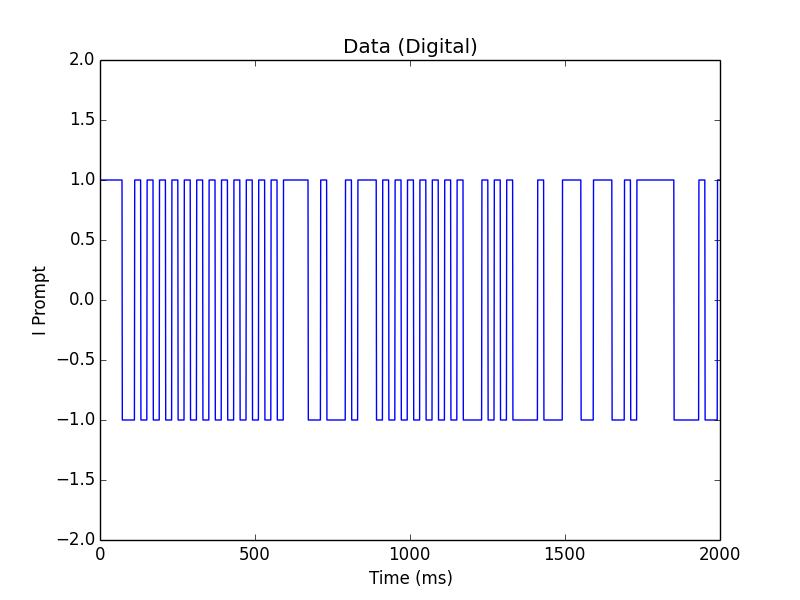
\includegraphics[width=1\textwidth]{mywork/3Digital.png} 
    \caption{This figure shows the same data as figure \ref{fig:RawSignal}, however the signal is discretized to either 1 or -1, allowing the digital signal to be more clearly seen.}
    \label{fig:DigitalSignal}
\end{figure}


\begin{figure}[!htb] 
    \centering
    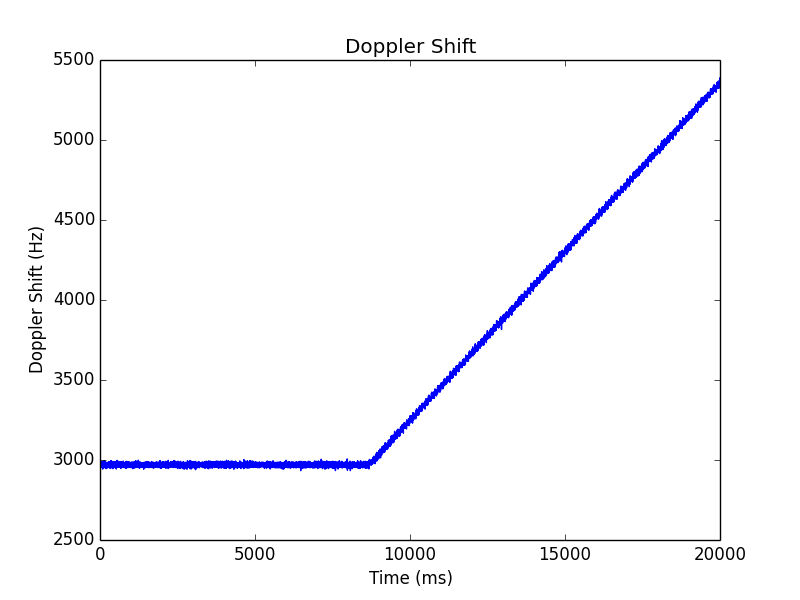
\includegraphics[width=1\textwidth]{mywork/22Doppler.png} 
    \caption{The \ac{NCO} doppler offset from the software receiver.}
    \label{fig:Doppler}
\end{figure}


A real-world data-set was processed, consisting of data taken aboard a flight aboard a UNSW Aviation Piper PA-44 Seminole. Data from the flight was captured by a NordNav IF Recorder, and processed using the python software receiver. 

The actual carrier doppler shift, as measured by taking the finite difference of the satellite pseudoranges, and converted to Hz, was compared against the measured Doppler shift in the software receiver. There is a small offset because of drift in the receiver crystal. The results of this experiment can be see in figure \ref{fig:SimulatedDynamics}. While the dynamics experienced by the receiver were on the order of $\pm 0.5g$, this experiment is important, as it verifies the real world performance of the system. 

\begin{figure}[!htb] 
    \centering
    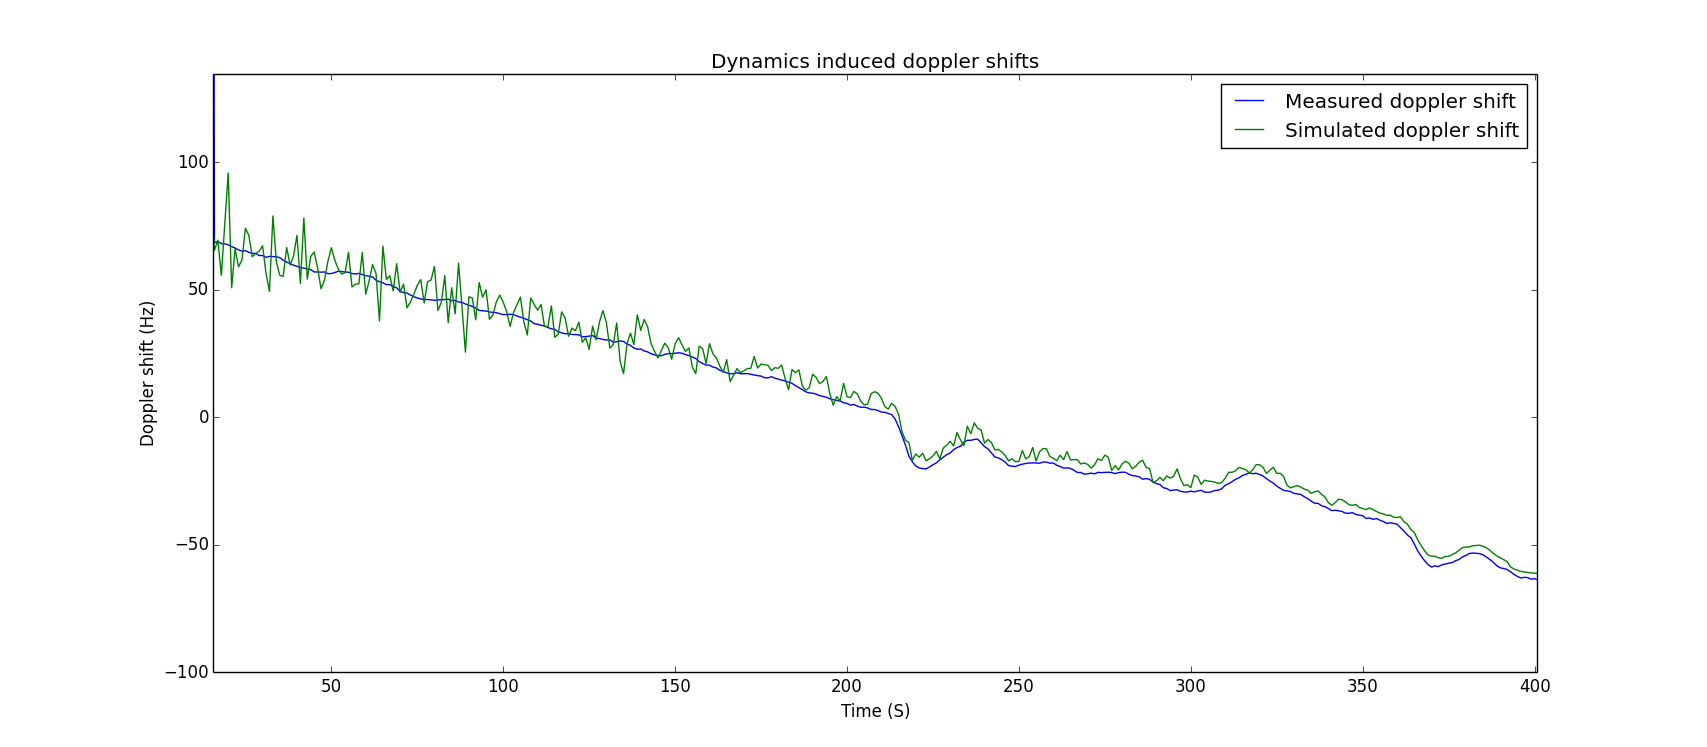
\includegraphics[width=1\textwidth]{mywork/SimulatedDynamics.png} 
    \caption{The python software receiver being tested on a real world data set. The constant offset is due to the drift in the receiver crystal.}
    \label{fig:SimulatedDynamics}
\end{figure}

\end{comment}
